\section{Dokumentation der Arbeitsweise}

\subsection{Tools}

\begin{itemize}
\item Git/GitHub: Versionskontrolle
\item Continuous Integration (Travis CI): Open-Source-Software für kontinuierliche
Integration
\item IntelliJ: Entwicklungsumgebung
\item JUnit: Framework zum Testen von Java-Programmen
\end{itemize}

\subsection{Vorgehen}

\begin{figure}[H]
	%\centering
	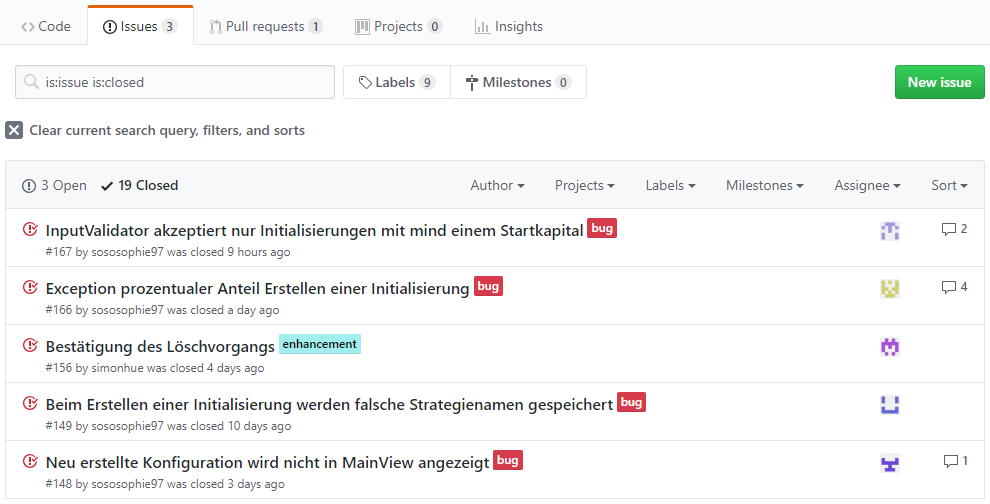
\includegraphics[width=1.1\textwidth]{qs_1.png}
	\caption{Übersicht der geschlossenen Issues auf GitHub}
\end{figure}